% Effects of Radiation

\documentclass[11pt]{article}

\usepackage[a4paper, margin=1in]{geometry}

\usepackage{amsmath}

\usepackage{amssymb}

\usepackage[german]{babel}

\usepackage[autostyle=true]{csquotes}

\usepackage{libertine}

\usepackage[libertine]{newtxmath}

\usepackage{tikz}

\usepackage{gensymb}

\usepackage{fancyhdr}

\usepackage{amsfonts}

\usepackage{pgfplots}

\pgfplotsset{compat=1.10}

\usepackage{multicol}

\usepackage{caption}

\usepackage{floatrow}

\everymath{\displaystyle}

% Header / footer settings

\pagestyle{fancy}
\fancyhf{}
\renewcommand{\headrulewidth}{0.2mm}
\fancyhead[C]{Funktionen}
\renewcommand{\footrulewidth}{0.2mm}
\fancyfoot[L]{Peter Goldsborough}
\fancyfoot[C]{\thepage}
\fancyfoot[R]{\today}

\fancypagestyle{plain}{%
	\fancyhf{}
	\renewcommand{\headrulewidth}{0mm}%
	\renewcommand{\footrulewidth}{0.2mm}%
	\fancyfoot[L]{Peter Goldsborough}
	\fancyfoot[C]{\thepage}
	\fancyfoot[R]{\today}
}


\setlength{\headheight}{15pt}

\setlength{\parindent}{0pt}

\addtolength{\parskip}{\baselineskip}


\newcommand{\overbar}[1]{\mkern 1.5mu\overline{\mkern-1.5mu#1\mkern-1.5mu}\mkern 1.5mu}

\newcommand{\heading}[1]{\begin{center}\Huge \textbf{#1}\end{center}\par}

\newcommand{\sub}[1]{\vspace{\parskip}{\LARGE\textbf{#1}}}

\newcommand{\subsub}[1]{{\Large \textbf{#1}}}

\newcommand{\subsubsub}[1]{\textbf{#1}}

\newcommand{\colvec}[1]{\begin{pmatrix}#1\end{pmatrix}}

\newcommand{\extrapar}{\par\vspace{\baselineskip}}

\newcommand{\zitat}[1]{\foreignquote{german}{#1}}

\newcommand{\bolditem}[1]{\item \textbf{#1}}

\newcommand{\titleitem}[1]{\bolditem{#1}\par}

\newcommand{\defas}{ \dots \,\,}

\begin{document}
\thispagestyle{plain}

\title{\Huge Effects of Radiation}

\author {
Peter Goldsborough\\
8A
}

\date{\today}

\maketitle

\textbf{\emph{Make a list of the main natural and man-made sources of background radiation.}}

\begin{itemize}
	\titleitem{Natural sources}

		\begin{itemize}
			\item Naturally occuring radioactive materials in
				  \begin{itemize}
				  		\item the earth's crust
				  		\item soil and stones
				  		\item walls and floors
				  		\item food and drinks
				  		\item our bodies' muscles, bones, tissue (Potassium 40, Carbon 14, Radium 22)
				  \end{itemize}
			\item Radioactive gases in the air, e.g. radon (Radon 222) thoron (Radon 220)
			\item Cosmic radiation / cosmic rays
		\end{itemize}

	\titleitem{Anthropomorphic sources}

		\begin{itemize}
			\item X-Rays
			\item Medical diagnosis --- Tracers, Scintigraphy, PET
			\item Nuclear explosvies testing
			\item Small leaks of radioactive material from coal or nuclear power plants
		\end{itemize}
\end{itemize}

\textbf{\emph{A useful measure for radiation exposure is the dose equivalent. How is it determined and what is its unit?}}

The \emph{dose of radiation} is a measure of the biological harm and effects of ionizing radiation on human tissue, measured in Sievert (Sv) $[1\frac{J}{kg}]$, named after the Swedish physicist Rolf Maximilian Sievert. One Sievert is a large quantity, so it is more usual to encounter millisievert (mSv) or microsievert ($\mu$sV). One chest X-Ray will give 0.2 mSv of radiation dose.

Another, non-SI unit of measurement is the \emph{rem} (roentgen equivalent in man). One rem is 0.01 sievert, so one sievert is 100 rem.

Actually, there are two different types of radiation doses and respective measurement units:

\begin{itemize}
	\bolditem{Absorbed dose} is a measure of the concentration of energy deposited in tissue as a result of an exposure to ionizing radiation. The absorbed dose is measured in Gray (gy) [$1\frac{J}{kg}$]. ``It is defined as the absorption of one joule of radiation energy by one kilogram of matter''. The US, non-SI equivalent measurement unit is one \emph{rad} (1 rad = 0.01 Gy).
	\bolditem{Equivalent dose} is the measure of the biological impact / damage of the absorbed dose on human tissue, measured in Sievert (Sv). The \emph{absorbed dose} describes the amount of energy [J] deposited in tissue by radiation exposure. The \emph{equivalent dose} measures the actual biological damage caused by the absorbed dose, as not all forms of radiation cause the same degree of damage.
\end{itemize}

\pagebreak

\textbf{\emph{Find out more about the average annual radiation exposure of a person due to background radiation. Which factors influence it? Which types of background radiation contribute the most?}}

The estimated average radiation dose received by a human per year is between 2.4 mSv and 3 mSv, though this can vary depending on altitude and latitude as well as geographical location. Especially the radiation dose from cosmic rays depends on altitude. People who live higher up or are frequent flyers are more exposed to cosmic radiation than others. The largest source of natural background radiation stems from varying amounts of uranium and thorium in the soil. Another noteworthy source is Radon in the air. Generally, two other factors that determine the radiation dose of any ionizing radioactive exposure are length (i.e. how long) and intensity of exposure. Figure \ref{fig:rem-chart} displays a chart with some average radiation dose values in rem. Table \ref{tbl:doses} displays some common radiation dose values encountered by humans per year or per exposure.

\begin{figure}[t!]
	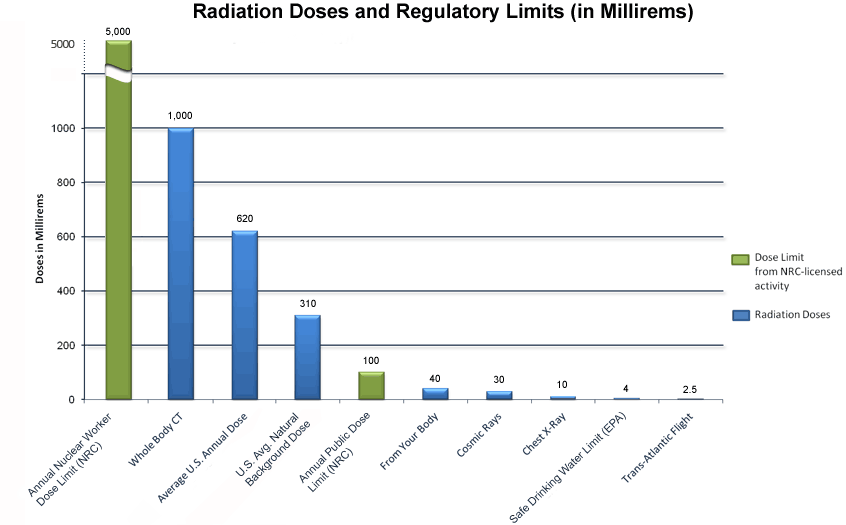
\includegraphics[scale=0.5]{img/rem-chart}
	\caption{Radiation doses in Millirems (1 rem = 0.01 Sv = 10 mSv; 1 millirem = 0.00001 Sv = 10 $\mu$Sv)}
	\label{fig:rem-chart}
\end{figure}

\begin{table}[h!]
\centering
	\begin{tabular}{|l|l|}
		\hline
		\rowcolor[gray]{0.8}
		Source & Dose (mSv)
		\\ \hline
		Radon gas & 2.3
		\\ \hline
		Solar and cosmic radiation & 0.3
		\\ \hline
		Diagnostic x-rays and nuclear medicine & 3.0
		\\ \hline
		Fallout from weapons testing & $<$ 0.01
		\\ \hline
		Nuclear industry & $<$ 0.01
		\\ \hline
		Airline travel & 0.001 - 0.014/h of flight
		\\ \hline
		Dental x-rays & 0.005
		\\ \hline
		Chest x-ray & 0.02
		\\ \hline
		Mammography & 0.4
		\\ \hline
		CT, head & 2
		\\ \hline
		CT, body (chest, abdomen, pelvis) & 6-8
		\\ \hline
	\end{tabular}
\caption{Radiation dose values per exposure or per year}
\label{tbl:doses}
\end{table}

\textbf{\emph{What effects does radiation exposure have on the human body? List some radiation dose values together with the resulting effects on the body.}}

Ionizing radiation exposure can cause biological harm to humans' tissue, by denaturing, harming or even killing cells. The reason for this is the $\alpha$ or $\beta$ particle and/or $\gamma$ ray decay as well as neutron emission resulting from nuclear radiation, which ionize tissue. Short-term effects include skin redness, hair loss, radiation burns, and acute radiation syndrome (ARS). Long-term consequences are mainly cancer or leukemia, the former being especially harmful to foetuses.

Table \ref{tbl:effects} lists some effects associated with certain radiation dose values.

\begin{table}[h!]
\centering
	\begin{tabular}{|p{3cm}|p{2cm}|p{2cm}|p{2cm}|p{2cm}|p{2cm}|}
		\hline 
		\rowcolor[gray]{0.8}
		Feature & 1-2 Gy & 2-6 Gy & 6-8 Gy & 8-30 Gy & $>$ 30 Gy
		\\ \hline
		Nausea and vomiting & 5-50\% & 50-100\% & 75-100\% & 90-100\% & 100\%
		\\ \hline
		Time of onset of nausea and vomiting after exposure & 2-6 h & 1-2 h & 10-60 min & $<$ 10 min & Minutes
		\\ \hline
		Severity and incidence of diarrhea & None & None to mild $<$0\%) &Heavy $>$0\%) & Heavy $>$5\%) & Heavy (100\%)
		\\ \hline
		Severity and incidence of headache & Slight & Mild to moderate (50\%) &Moderate (80\%) & Severe (80-90\%) & Severe (100\%)
		\\ \hline
		Severity of fever & None & Moderate increase & Moderate to severe & Severe & Severe
		\\ \hline
		Acute mortality without medical care & 0-5\% & 5-100\% & 95-100\% & 100\% & 100\%
		\\ \hline
		Acute mortality with medical care & 0-5\% & 5-50\% & 50-100\% & 100\% &100\%
		\\ \hline
		Death & 6-8 wk & 4-6 wk & 2-4 wk & 2 days-2 wk & 1-2 days
		\\ \hline
	\end{tabular}
\caption{Radiation dose values and their consequent biological effects on the human body}
\label{tbl:effects}
\end{table}

\textbf{\emph{How can food, in general, become contamined with radioactive materials? Which effects does the consumption of contamined food have on the human body?}}

Causes for the radioactive contamination of food, such as vegetables, fruits, animals or fodder, include radioactive material in the air, rain water, snow or soil, which is then transferred to crops or animals. Radioactivity can also be washed into rivers, lakes and the sea where fish and seafood could take up the radionuclides.

The potential health risks and consequences of consuming radioactively contaminated food generally include an increased level of exposure, carrying with it all the effects of such radiation, such as a higher risk of cancer, particularly in children. The main contaminants in food are radioactive iodine and caesium, the former of which can cause thyroid cancer. Event though iodine has a half-life of eight days and decays naturally within weeks, it can accumulate in the body. 

\pagebreak

\textbf{\emph{Which radionuclides, set free by the accident in Fukushima's nuclear power plant, are most dangerous for humans? Find out more about them (half-life, type(s) of radiation given off, transformation equation, effects on the body).}}

The most important and most dangerous radionuclides released in the course of the Fukushima-Daiichi accident are Iodine I-131, Caesium Cs-134 and Cs-137, though also levels of Plutonium, Tritium H-3 and Iodine I-129 have been measured. Table \ref{tbl:nuclides} gives a selection of properties of the most important radionuclides.

\begin{table}[b!]
\centering
	\begin{tabular}{| p{2.5cm} | l | p{2cm} | p{3cm} | p{4cm} |}
		\hline 
		\rowcolor[gray]{0.8}
		Radionuclide & Half-life & Radiation & Transformation equation & Effects on the body
		\\ \hline
		Iodine $\ce{^{131}_{53}I}$ & 8.02 days & $\beta^- + \gamma$ & ${^{131}_{53}\ce{I}} \rightarrow \beta^- + \bar{\nu_e} + \ce{^{131}_{54}Xe}  + 606 keV$ & Risk of thyroid cancer due to accumulation in thyroid gland after radioactive fallout or food contamination
		\\ \hline
		Caesium $\ce{^{134}_{55}Cs}$ & 2.01 years & $\beta^- + \gamma$ & $ \ce{^{134}_{55}Cs} \rightarrow \beta^- + \bar{\nu_{e}} + \ce{^{134}_{56}Ba} + 698 keV$ & Exposure can be toxic and is associated with an increased risk of cancer, especially for infants or foetuses. Radioactive cesium can accumulate in water as well as plant tissues, including fruits, vegetables, and mushrooms, potentially compromising the food and water supply.
		\\ \hline
		Caesium $\ce{^{137}_{55}Cs}$ & 30.17 years & $\beta^- + \gamma$& $\ce{^{137}_{55}Cs} \rightarrow \beta^- + \bar{\nu_{e}} + \ce{^137_{56}Ba} + 1176 keV$ & Caesium-137 can react with water to create caesium hydroxide. When entering the body, it is distributed uniformly, with high concentrations in soft tissue, so the decay is harmful in all areas.
		\\ \hline
	\end{tabular}
\caption{Noteworthy radionuclides set free during the Fukushima reactor incident and their respective properties}
\label{tbl:nuclides}
\end{table}

\pagebreak

\textbf{\emph{What can you do to reduce the risk of contamination with radioactive substances in case of a nuclear power station accident? How can you protect yourself when working with radioactive substances?}}

Means of reducing the risk of radioactive contamination and nuclear fallout, as well as personal protective measures during the early phase of a nuclear emergency, include:

\begin{itemize}
	\item Staying informed and keeping accurate information about the current situation through radio, television or the internet, to be able to follow governments' and experts' instructions.
	\item Taking Potassium Iodide pills containing stable, non-radioactive iodine which saturates the thyroid gland so it blocks the intake and accumulation of radioactive iodine which can cause (thyroid) cancer. Does not protect against contamination or radiation. Another antidoe is Prussian Blue.
	\item Stay clean and bathe / wash with soap to get rid of contamination on skin. 
	\item Throw away (possibly) contaminated clothes.
	\item Try to get out of the contaminated area as quickly as possible, find a safe building where you have access to help from law enforcement, health officials or other authorities.
\end{itemize}

To protect yourself when handling radioactive substances, you should:

\begin{itemize}
	\item Keep as much distance as possible, as radiation exposure intensity increases the closer you are to the radioactive substance
	\item Try to limit the exposure time
	\item Appropriate shielding for the radiation emitted:
		\begin{enumerate}
			\item $\alpha \rightarrow$ clothing suffices for external body areas, but tissue inside the body must be protected at all costs to prevent tissue damage and denaturing by internal alpha radiation.
			\item $\beta \rightarrow$ additional heavy clothing to protect skin and outside of the body, as $\beta$ radiation can penetrate and burn the skin.
			\item $\gamma \rightarrow$ thick shielding such as lead or thick concrete must be used, as $\gamma$ rays have extremely high energy and can penetrate almost anything and thus easily damage biological tissue inside and outside the human body.
		\end{enumerate}
\end{itemize}

\sub{Sources}

\begin{enumerate}
	\item \href{http://www.radiologyinfo.org/en/safety/index.cfm?pg=sfty_hiw_09}{http://www.radiologyinfo.org/en/safety/index.cfm?pg=sfty\_hiw\_09}
	\item \href{http://www.merckmanuals.com/professional/injuries_poisoning/radiation_exposure_and_contamination/radiation_exposure_and_contamination.html}{http://www.merckmanuals.com/professional/injuries\_\\poisoning/radiation\_exposure\_and\_contamination/radiation\_exposure\_and\_contamination.html}
	\item \href{https://www.iaea.org/sites/default/files/seafoodsafety0511_0.pdf}{https://www.iaea.org/sites/default/files/seafoodsafety0511\_0.pdf}
	\item \href{https://www.iaea.org/node/10898}{https://www.iaea.org/node/10898}
	\item \href{http://www.who.int/hac/crises/jpn/faqs/en/index.html}{http://www.who.int/hac/crises/jpn/faqs/en/index.html}
	\item \href{http://en.wikipedia.org/wiki/Isotopes_of_caesium}{http://en.wikipedia.org/wiki/Isotopes\_of\_caesium}
\end{enumerate}

\end{document}